\section{Metodologia}

Todo o estudo proposto será realizado seguindo a metodologia Cross Industry Standard Process for Data Mining - CRISP-DM \cite{chapman2000crisp}, que é um processo padrão para mineração de dados.

O CRISP-DM envolve um ciclo faseado para um projeto ou pesquisa de mineração de dados, conforme apresentado na Figura \ref{fig1}:

\begin{figure}[htbp]
	\centerline{
		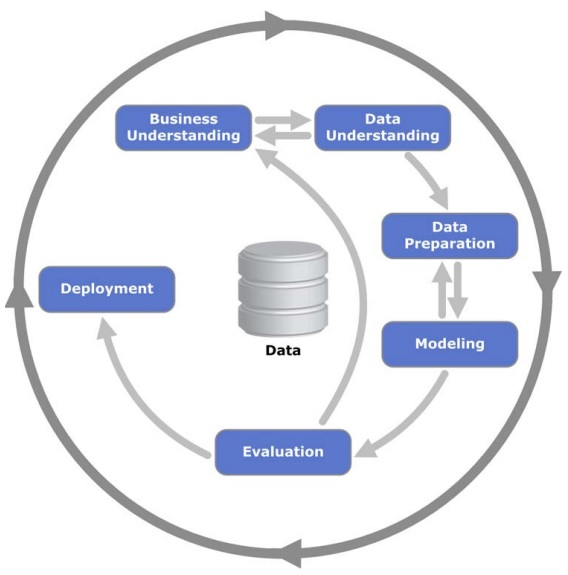
\includegraphics[width=80mm,scale=0.8]{assets/crispdm.jpg}
	}
	\caption{Phases of the CRISP-DM Process Model}
	\label{fig1}
\end{figure}

Os passos do CRISP-DM são:

\begin{enumerate}
	\item Compreensão do negócio: nesta etapa, o contexto do problema apresentado será analisado com detalhe para uma melhor compreensão da vulnerabilidade feminina.
	\item Compreensão dos dados: nesta etapa, os dados do RAIS serão coletados e examinados para identificar problemas de qualidade e verificar se eles são adequados para atender aos objetivos da pesquisa. Além disso, serão identificadas as variáveis que serão utilizadas na análise.
	\item Preparação dos dados: nesta etapa, os dados da RAIS serão preparados para análise, o que pode incluir a limpeza de dados, a transformação de variáveis e a seleção de subconjuntos de dados relevantes. 
	\item Modelagem: nesta etapa, serão aplicados modelos estatísticos ou de aprendizado de máquina para identificar padrões nos dados da RAIS, bem como relações entre variáveis.
	\item Avaliação: nesta etapa, os resultados da modelagem serão avaliados para verificar se eles atendem aos objetivos da pesquisa, isto é, se eles fornecem informações úteis.
	\item Implantação: nesta etapa final, os resultados serão apresentados e as hipóteses confirmadas ou refutadas.     	      	      	      	      	      
\end{enumerate}

  